\chapter{Implementierung der Betriebssoftware}
Die Betriebssoftware wurde, wie in der Aufgabenstellung festgelegt, in C geschrieben.
Hierbei fiel die Wahl auf den Standard C99, der gegenüber C89 einige sprachliche
Aktualisierungen aufweist. Als Compiler wurde eine Version der
GNU-Compiler-Collection (GCC) mit einem Backend für AVR-kompatiblen Assembler benutzt.
Außer der C-Standard-Library und der AVR-IO-Library besitzt die Software keine externen
Abhängigkeiten im Code.

\section{Die Hauptschleife}
Die Hauptschleife ist in dieser Implementierung eine Endlosschleife, da die Beendigung dieser
Schleife sonst dazu führen würde, dass das System nicht mehr reagiert.
Wie in Abb. \ref{impl_main_loop} zu sehen ist, werden in der Hauptschleife vier wichtige Funktionen
aufgerufen.
\begin{figure}[h]
 \centering
 \scalebox{0.5}{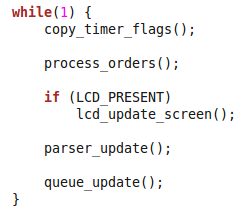
\includegraphics{pictures/main_loop_code.png}}
 \caption{\label{impl_main_loop}Die Hauptschleife}
\end{figure}

\subsection{process\_orders()}
Die process\_\-orders()\--Funktion bearbeitet die Befehle, die bereits in der Queue sind. Dafür holt
sich die Funktion den aktuellen Befehl von der Queue. Wenn es solch einen Befehl gibt, ruft die
Funktion eine Verteilerfunktion auf. Diese wiederum ruft die zugehörige Befehlsfunktion auf, indem
der Befehlscode als Index für eine Call-Table benutzt wird (siehe
Abb. \ref{dispatch_function}).\\
\begin{figure}[htb]
 \centering
 \scalebox{0.6}{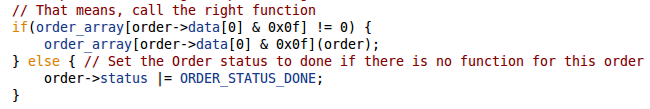
\includegraphics{pictures/dispatch_function.png}}
 \caption{\label{dispatch_function}Die Verteilerfunktion}
\end{figure}
Falls kein Befehl vorliegt, oder die Queue angehalten wurde, ruft die process\_\-orders()-Funktion die
Funktion zum aktiven Bremsen auf. Das aktive Bremsen wird in Kapitel \ref{chapter_abs} behandelt.

\subsection{lcd\_update\_screen()}
Wenn ein LCD angeschlossen ist, können dort Informationen ausgegeben werden.
Der Anschluss des LCD wird dem System mit einem DIP-Schalter auf der Platine mitgeteilt.\\
Da das synchrone Aktualisieren des LCD sehr viel Zeit benötigt (vgl. Kapitel \ref{chapter_lcd_problem}), wird
pro Aufruf dieser Funktion maximal ein Zeichen an das LCD geschickt.
Dies wird durch Abfrage des Busy-Flags erreicht, welches signalisiert, dass das LCD noch
beschäftigt ist. Falls es nicht gesetzt ist und noch Daten zu aktualisieren sind,
wird das nächste Zeichen an das LCD gesendet.\\
Auf dem LCD werden die Versionsnummer der Betriebssoftware, der Status einiger globaler Variablen und
der aktuell ausgeführte Befehl angezeigt. Wenn nun ein Befehl bearbeitet wird, der länger als einen
Schleifendurchlauf benötigt (das sind z.B. alle Fahr-Befehle), ruft die lcd\_\-update\_\-screen()-Funktion
die lcd\_\-update\_\-info()-Funktion auf, die diese Informationen in einem Puffer konstruiert. Nach und nach
gibt die lcd\_\-update\_\-screen()-Funktion den Inhalt dieses Puffers an das LCD weiter.\\
Befehle, die innerhalb eines Hauptschleifendurchlaufs abgearbeitet sind, werden nicht ausgegeben und
generieren auch keinen Aufruf von lcd\_\-update\_\-info(). Das ist nötig, weil diese Befehle zu schnell abgearbeitet
werden. Es könnten zwischenzeitlich vier bis fünf dieser Befehle abgearbeitet werden, bevor das LCD auch nur einmal vollständig
aktualisiert werden kann.

\subsection{parser\_update()}
Der Parser ist dafür zuständig, aus den Bytes, die über I2C oder UART gelesen werden, Befehle in Form von
order\_t-Strukturen zu erstellen. Die parser\_\-update()-Funktion fragt beim IO-Modul nach, wie viele Bytes
zum Abholen bereit stehen. Diese werden dann geholt und an die Funktion parser\_\-add\_\-byte() übergeben.\\
Diese parser\_\-add\_\-byte()-Funktion fügt das Byte an die richtige Stelle im Puffer ein. Wenn ein Befehl
komplett ist, dies wird mit der parser\_\-order\_\-complete()-Funktion überprüft, gilt der Befehl als fertig und
alle weiteren Bytes, die hinzugefügt werden, landen in einer neuen order\_t-Struktur.\\
Zum Erkennen, wann ein Befehl zu Ende ist, benutzt die parser\_\-order\_\-complete()-Funktion
die bytes\_\-needed()-Funktion. In dieser ist fest codiert, welcher Befehlscode mit welchen Optionen wie viele
Bytes benötigt. Das ist auch eine der Stellen, die angepasst werden müssen, wenn neue Befehle hinzugefügt
oder bestehende verändert werden sollen.

\subsection{queue\_update()\label{chapter_queue_update}}
Diese Funktion führt Wartungsarbeiten an der Befehlswarteschlange (Queue) durch. Das beinhaltet, neue
Befehle beim Parser-Modul abzuholen und diese korrekt einzureihen. Es gibt zwei Möglichkeiten, wie die
neuen Befehle an die Queue angereiht werden können. Zum einen als normale Befehle, die einer nach dem anderen abgearbeitet werden,
zum anderen als priorisierter Befehl. Es kann nur ein priorisierter Befehl in der Queue sein. Die Befehle werden
umgehend in der nächsten Haupt\-schleifen\-iteration ausgeführt. In die Kategorie der priorisierten Befehle fallen
alle Queue-Kontroll-Befehle, wie z.B. pausieren, löschen, aktuellen Befehl verwerfen etc. (vgl. Kapitel \ref{chapter_protokoll}).

\section{Das Aktive-Brems-System (ABS)\label{chapter_abs}}
Das aktive Bremssystem soll bewirken, dass die Räder im praktischen Betrieb ihre Position nicht verlassen können.
Dies wird realisiert, indem
eine Referenz-Position für jedes Rad gespeichert wird. Während der Hauptschleife wird die tatsächliche Position mit
der Referenz-Position verglichen. Für den Fall, dass diese Positionen nicht übereinstimmen, werden die Motoren mit einer
einstellbaren Geschwindigkeit so betrieben, dass die Räder wieder auf die Referenz-Position gebracht werden.\\
Die Referenz-Positionen werden an drei verschiedenen Stellen im Code gesetzt. Zum einen in der process\_\-orders()-Funktion
in der Hauptschleife, wenn der aktuelle Befehl beendet wurde, zum anderen in den Fahr-Befehls-Funktionen, falls ein Rad
früher als das andere seine Stopp-Bedingung erreicht hat.\\
Das ABS kann vom Benutzer bei laufendem System angepasst werden. So kann man die Geschwindigkeit ändern, mit der
die Motoren die Positions-Differenz ausgleichen. Außerdem kann man Teile des ABS deaktivieren oder auch reaktivieren,
oder das gesamte ABS abschalten bzw. wieder anschalten. So kann der Benutzer das ABS an seine Wünsche anpassen.

\section{Befehle: Struktur und Funktionen}
Die Struktur (Abb. \ref{order_type}), die einen Befehl im System repräsentiert, besteht hauptsächlich aus einem Array, in dem die eigentlichen Daten
gespeichert sind, und einem Status-Byte, in dem Statusinformationen in Form von Flags gespeichert werden.
\begin{figure}[htb]
 \centering
 \scalebox{0.6}{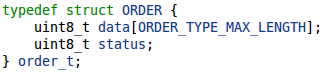
\includegraphics{pictures/order_t.png}}
 \caption{\label{order_type}Befehlsstruktur}
\end{figure}
Das erste Byte dieses Arrays ist das Kommando-Byte, welches die Art des Befehls und die zugehörigen Optionen spezifiziert. Der
Befehlscode 0x00 ist für zukünftige Erweiterungen reserviert, die mehr als ein Kommando-Byte
benötigen. Des Weiteren sind die Befehlscodes 0x01 bis 0x06 durch diese Arbeit bereits definiert und mit Funktionalität erfüllt.
Die Befehlscodes 0x07 bis 0x0f sind noch nicht definiert und können für zukünftige Erweiterungen benutzt werden, die mit \textbf{einem}
Kommando-Byte auskommen.\\
Alle auf das Kommando-Byte (oder die Kommando-Bytes im Falle des Befehlscodes 0x00) folgenden Bytes sind Parameter. Deren Anzahl und Länge
hängt von der Spezifikation des Befehls ab.
Bei Parametern, die länger als ein Byte sind, wird zuerst das höchstwertige Byte im Array gespeichert. 
Dann folgen die übrigen Bytes mit absteigender Wertigkeit.\\
Oft benutzte Aktionen bezüglich der Befehlsstruktur wurden zusammengefasst (siehe Abb. \ref{order_init} und \ref{order_copy}).
Vor der Untersuchung des Laufzeitverhaltens, und der damit einhergehenden Optimierungen, wurden diese beiden Funktionen
durch for-Schleifen implementiert. Wie sich bei der Untersuchung herausstellte, waren die for-Schleifen aber langsamer
als die Standard-C-Funktionen memset() und memcpy().
\begin{figure}[htb]
 \centering
 \scalebox{0.6}{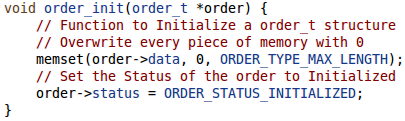
\includegraphics{pictures/order_init.png}}
 \caption{\label{order_init}order\_init()-Funktion}
\end{figure}
\begin{figure}[htb]
 \centering
 \scalebox{0.6}{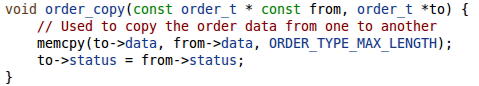
\includegraphics{pictures/order_copy.png}}
 \caption{\label{order_copy}order\_copy()-Funktion}
\end{figure}

\section{Datenpfad von Befehlen}
Befehle werden entweder über die UART- oder die I2C-Schnittstelle byteweise empfangen. Diese Schnittstellen werden über
Interrupt-Service-Routinen bearbeitet, um zeitnah auf eingehende Daten zu reagieren, da diese Übertragung die größte
Latenz-Quelle darstellt (I2C: ca. 270 \textmu{}s pro Byte; UART: ca 139 \textmu{}s pro Byte). In diesen Interrupt-Service-Routinen wird
das empfangene Byte in den Eingangspuffer gelegt. Wenn die Hauptschleife wieder die parser\_\-update()-Funktion erreicht,
werden die bisher empfangenen Bytes abgeholt und in dem Parser-Puffer abgelegt, um aus den Bytes order\_t-Struktur-Instanzen
zu generieren. Wenn der Befehl fertig im Parser vorliegt, ruft ihn queue\_\-update() ab und reiht ihn in die Warteschlange
ein (siehe Kapitel \ref{chapter_queue_update}). Von der Warteschlange holt sich die process\_\-orders()-Funktion den
aktuellen Befehl und führt die zugeordnete order\_function-Funktion solange aus, bis im Status-Byte (vgl. Abb. \ref{order_type})
das ORDER\_\-STATUS\_\-DONE-Flag gesetzt wurde. Anschließend entfernt sie diesen aus der Warteschlange.\\
Falls der zu bearbeitende Befehl eine Ausgabe von Daten bewirkt, werden diese in der entsprechenden order\_\-function-Funktion
in dem Ausgabepuffer des IO-Frameworks angereiht. Dieses Framework wird dann, sobald wie möglich, diese Daten
über die ausgewählte Schnittstelle senden (bei UART wird sofort mit dem Senden begonnen; bei I2C muss gewartet werden, bis die Daten
vom Benutzer abgerufen werden).
% Datenpfadbild

\section{Debug-Ausgaben \label{impl_debug}}
Es ist nicht ohne weiteres möglich, einen üblichen Debugger zur Fehlerfindung zu verwenden; stattdessen
sind Debug-Ausgaben notwendig, um die Funktion des Debuggers zu ersetzen.
Im Gegensatz zu einem Debugger muss zusätzlicher Programmcode eingefügt werden, um Debug-Ausgaben
realisieren zu können.
Diese Ausgaben beeinträchtigen die Geschwindigkeit des gesamten Systems auch dann noch, wenn
diese mit if-Statements umschlossen werden (siehe Abb. \ref{debug_trick}).

Während der normalen Operation der Betriebssoftware im Praktikum sind diese Ausgaben
nicht nötig, und für die meisten Teilnehmer des Praktikums nicht informativ.
Der Leser muss eine entsprechende Kenntnis des Codes besitzen, damit die Ausgaben
für die Fehlerbehebung benutzt werden können.\\
Wegen der geringen Hilfe, die diese Ausgaben im Normalfall dem Praktikanten bieten,
und der negativen Auswirkung der Ausgaben auf die Performance des Systems, wurde
eine Prä-Prozessor-Technik angewandt, die zusammen mit der eingestellten Stufe der
Code-Optimierung des Compilers die beiden Probleme löst.

Durch diese Technik werden die Debug-Ausgaben nur dann kompiliert,
wenn dem Compiler der Parameter -DDEBUG übergeben wird. 
Zwar ist es auch dann noch möglich, mit einem DIP-Schalter auf der Platine die Ausgaben
auszuschalten, aber es bleiben immer noch die leicht negativen Auswirkungen auf die Performance.

Normalerweise
wird die Betriebssoftware ohne diesen Parameter kompiliert. Das bedeutet, dass die Software neu kompiliert werden muss, wenn
diese Debug-Ausgaben erwünscht sind.
\begin{figure}[htb]
 \centering
 \scalebox{0.5}{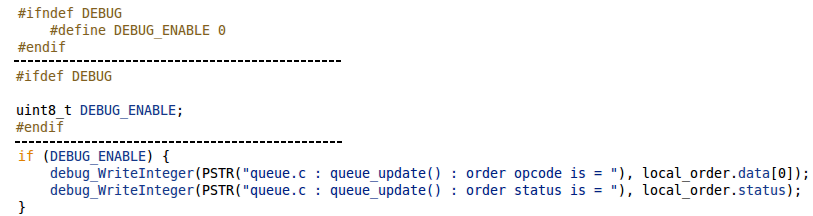
\includegraphics{pictures/debug_trick.png}}
 \caption{\label{debug_trick}Debug-Defines und die Verwendung im Code}
\end{figure}

\section{IO-Framework}
Das Ziel des IO-Frameworks war die Abstraktion der Ein- und Ausgabe von Daten der zu Grunde liegenden Schnittstellen.
Die UART- und die I2C-Schnittstelle sind in der Benutzung sehr unterschiedlich. Statt überall im Code, wo E/A stattfindet,
jeweils für beide Schnittstellen Code einzufügen, wurde das IO-Framework als Zwischenschicht entwickelt. Es verfügt sowohl
über einen Ausgabe- als auch einen Eingabepuffer. Diese sind jeweils auf 256 Bytes festgelegt. Durch diese Definition
konnte das normale Überlaufverhalten der 8-Bit-Variablen ausgenutzt werden, um Modulo-Operationen zu ersetzen, welche
unangemessen viel Zeit in Anspruch nehmen.\\
Eine Besonderheit ist die Ausgabe von Daten auf Objekt-Basis. Ein Objekt hat mindestens ein Byte und maximal 256 Byte. Objekte
werden entweder komplett übertragen oder gar nicht. Wenn ein Objekt nicht komplett übertragen werden konnte, wird bei der
nächsten Übertragung vom Anfang des Objektes wieder angefangen. Außerdem bewirkt die Ausgabe von Objekten bei Benutzung der
I2C-Schnittstelle, dass für jede Lese-Operation, die von der Praktikumsplatine eingeleitet wird, ein Objekt übermittelt wird.\\
E/A-Operationen geschehen nicht-blockend und gepuffert. Damit verbraucht die E/A nur Prozessorzeit, wenn es nötig ist, und
vermeidet so nutzlosen Zeitverbrauch bedingt durch aktives Warten.

\section{Unterstützende Bibliothek für die Praktikumsplatine}
Die Benutzung der Motorplatine soll für die Studierenden möglichst einfach sein.
Aus diesem Grund wurde neben der Betriebssoftware für die Motorplatine auch eine
Bibliothek für die Praktikumsplatine geschrieben. Diese Bibliothek stellt
Funktionen und Definitionen zur Verfügung, um Befehle an die Motorplatine
senden oder empfangen zu können. Hierfür wurde eine modifizierte Version der
Befehls-Struktur für die Praktikumsplatine geschrieben. Es sind drei Funktionsaufrufe
nötig, um jeden möglichen Befehl zusammenzustellen und zu versenden. Die erste
Funktion setzt das Kommando-Byte. Die zweite setzt die Parameter; dies wurde
mit einer Funktion gelöst, die eine variable Liste von Argumenten erhält. Die dritte und
letzte Funktion sendet den Befehl an die Motorplatine. Vorher muss allerdings die
Befehls-Struktur einmal initialisiert werden.
\begin{verbatim}
order_t order;
order_init(&order);
order_set_type(&order, ORDER_DRIVE_P_P);
order_add_params(&order, "1122", 127, -100, 32700, 16768);
order_send(&order);
\end{verbatim}
